\documentclass[../ai_in_finance]{subfiles}
\usepackage[margin=1in]{geometry}
\usepackage{tikz}
\usetikzlibrary{positioning}
\usepackage{amsmath}
\usepackage{amssymb}
\usepackage{booktabs}
\usepackage{floatrow}
\usepackage{draftwatermark}

\SetWatermarkText{Wulin.Suo@Queensu.ca}
\SetWatermarkScale{1.4}
\SetWatermarkColor{gray!35}
\SetWatermarkAngle{45}

\usepackage{makeidx}
\makeindex

\begin{document}

\chapter{Operational Risk Modeling}

\section{Introduction}

In January 2008, Société Générale disclosed a loss of roughly 4.9 billion euros. No market view had been wrong, no borrower had defaulted, and no model had mispriced a derivative. A single trader on the bank's arbitrage desk, Jérôme Kerviel, had built enormous unauthorized directional positions and concealed them behind offsetting fictitious trades that the bank's own controls failed to catch until the positions had to be unwound into a falling market. The loss was not a market-risk loss or a credit-risk loss in the sense of the previous two chapters. It was an \emph{operational} loss: a failure of the bank's internal processes, systems, and people.

Chapter 8 developed the machinery for market risk, how much a position's value could move, and Chapter 9 developed the machinery for credit risk, whether a counterparty will pay at all. This chapter turns to the risk that is left over once those two are accounted for, and that neither of their toolkits handles well: the risk of loss from failed internal processes, people, systems, or external events. Operational risk\index{operational risk} is at once the most intuitive of the three, everyone understands a rogue trader\index{rogue trading} or a systems outage, and the hardest to model, because its events share almost none of the statistical regularity that makes market and credit risk tractable.

It would be a mistake to treat operational risk as a minor residual. For many large banks it consumes a comparable share of regulatory capital to market risk, and its worst realizations, the multi-billion-dollar rogue-trading losses, the mis-selling scandals that end in nine- and ten-figure settlements, the systems failures that halt a payment network, have brought down or nearly brought down major institutions in a way a bad week of trading rarely does. What makes it distinctive is not its size but its character: where market and credit losses arrive through prices and defaults that the previous two chapters could model with dense data, operational losses arrive through the failure of the institution's own machinery, and the data on those failures is scarce, messy, and mostly unstructured.

That difficulty is why this chapter is worth a careful treatment in a book about artificial intelligence in finance, and why its central message is a nuanced one rather than a triumphant one. Artificial intelligence does not hand operational risk the kind of clean predictive model it hands credit scoring or volatility forecasting. What it does instead is asymmetric: it is genuinely powerful in the layers of the problem that are made of unstructured data and rare-pattern detection, reading incident reports, flagging anomalous behavior, surveilling for misconduct, warning early from leading indicators, and genuinely limited in the layer that regulators care most about, putting a credible number on the far tail. Keeping that asymmetry in view is the discipline this chapter is built around.

The chapter proceeds in three movements. It first establishes what operational risk is and why it resists a unified statistical model, then develops the classical actuarial baseline, the loss distribution approach, that any AI method must be measured against. It then works through the four layers where machine learning genuinely contributes, text, anomaly detection, conduct surveillance, and predictive early warning, each reusing methods this book has already developed, before turning reflexively to the ways deploying AI itself \emph{creates} new operational risk, and closing with the regulatory reason AI's natural home here is risk management rather than regulatory capital.

\section{What Operational Risk Is, and How It Is Measured}

Operational risk resists a single model, and this part explains why, then builds the loss distribution anyway.

\subsection{What Operational Risk Is, and Why It Resists a Single Model}
\label{sec:oprisk-fundamentals}

The Basel Committee defines operational risk as the risk of loss resulting from inadequate or failed internal processes, people, and systems, or from external events. The definition is deliberately broad, and it is conventionally organized into seven event-type categories\index{Basel operational-risk event types}, shown in Table~\ref{tab:oprisk-event-types}, that span everything from a rogue trader to a flooded data center.

\begin{table}[htbp]
\centering
\begin{lrbox}{\bookmeasuredbox}
\begin{tabular}{p{6.0cm}p{7.6cm}}
\toprule
Event type & Representative event \\
\midrule
Internal fraud & A trader conceals unauthorized positions \\
External fraud & A third party breaches systems and steals funds \\
Employment practices \& workplace safety & A discrimination or wrongful-termination settlement \\
Clients, products \& business practices & A mis-sold product or a market-manipulation fine \\
Damage to physical assets & A fire or natural disaster destroys a facility \\
Business disruption \& system failures & A core banking outage halts settlement \\
Execution, delivery \& process management & A failed trade settlement or data-entry error \\
\bottomrule
\end{tabular}
\end{lrbox}
\ifdim\wd\bookmeasuredbox<0.65\linewidth
\setlength{\bookcapwidth}{0.65\linewidth}
\else
\setlength{\bookcapwidth}{\wd\bookmeasuredbox}
\fi
\floatbox[\capbot]{table}[\bookcapwidth]{
\usebox{\bookmeasuredbox}
}{
\caption{The seven Basel operational-risk event types, with representative losses}
\label{tab:oprisk-event-types}
}
\end{table}

What makes this list so awkward to model is precisely that its rows share so little in common. A market-risk desk has a long, dense history of daily returns; a credit portfolio has thousands of loans with observable defaults. Operational risk has neither. Its defining events are \emph{rare}, so any single institution observes only a handful of large losses in its entire history; \emph{heavy-tailed}, so the few large events dominate the total and the average loss is a poor guide to the extreme one; \emph{heterogeneous}, so a rogue-trading loss and a mis-selling fine and a data-center fire have no common driver a single model could exploit; and subject to severe \emph{reporting and survivorship bias}, since near-misses go unrecorded, small losses are absorbed silently, and the institutions that suffer the very largest losses sometimes do not survive to contribute them to any database.

A further complication, invisible in the flat list of Table~\ref{tab:oprisk-event-types}, is that the event types differ enormously in their frequency-severity profile, and in opposite directions. Execution, delivery, and process-management errors are the most \emph{frequent}, a mistyped settlement, a duplicated payment, a reconciliation break happens daily at a large bank, but each is individually small. Clients, products, and business-practices events, mis-selling, market-conduct violations, large regulatory settlements, are comparatively \emph{rare} but individually enormous, and at most large banks they dominate total operational losses by value despite being a small fraction of events by count. A model or a control program calibrated to the frequent-but-small failures will therefore miss most of the actual loss, which lives in the rare-but-huge category, one more reason the tail, not the average, is where operational-risk attention belongs.

This is the same conclusion Chapter 9 reached when it introduced operational-risk capital from the credit side: a rogue trader's unauthorized position, a failed core-banking upgrade, and a mis-sold product ``share so little common structure that no single statistical framework fits all of them well.'' That is not a gap this book is about to close with a neural network. It is the fixed constraint within which every method in this chapter, classical or AI, has to operate.

\subsection{The Four Data Elements of Operational Risk}
\label{sec:oprisk-data}

Because no single data source captures operational risk well, the discipline conventionally draws on four distinct elements, and understanding them explains both where the loss model of the next section gets its inputs and where artificial intelligence has the most to add.

\emph{Internal loss data}\index{internal loss data} is a bank's own history of realized operational losses, the primary input to the frequency and severity estimates of Section~\ref{sec:oprisk-lda}, but it is sparse, especially in the tail, and skewed toward the small, frequent losses that are least relevant to capital. \emph{External loss data} is drawn from consortium databases of losses suffered by peer institutions, supplementing the tail with events a single firm has been fortunate enough not to experience, at the cost of relevance, since another firm's loss may reflect a control environment nothing like one's own. \emph{Scenario analysis}\index{scenario analysis} fills the remaining gap with structured expert judgment: workshops in which experienced staff estimate the frequency and severity of severe hypothetical events that have not occurred but plausibly could, the only element that can speak to genuinely unprecedented tail risk. \emph{Business environment and internal control factors} are the forward-looking indicators, the key risk indicators of Section~\ref{sec:oprisk-kri} among them, that describe the current control environment rather than past losses.

Three of these four elements are, in large part, text and expert judgment rather than clean numbers, which is precisely why the natural-language and classification methods of this chapter matter so much: the incident narratives behind internal loss data, the free-text descriptions in external databases, and the qualitative reasoning of scenario workshops are all unstructured, and turning them into model inputs is the AI-heavy part of operational-risk practice. The actuarial machinery of the next section is only as good as the data these four elements feed it, and its most common failure in practice is not a flaw in the mathematics but a thin, biased, or miscategorized loss dataset underneath it. Figure~\ref{fig:oprisk-data-elements} shows how the four elements combine to feed both the quantitative loss model and the qualitative control assessment.

\begin{figure}[htbp]
\centering
\begin{lrbox}{\bookmeasuredbox}
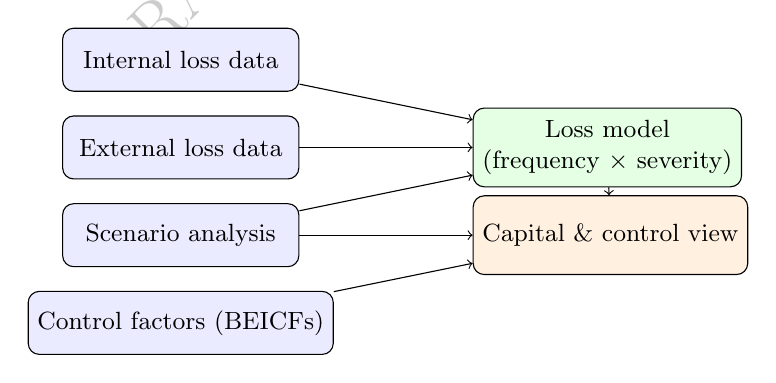
\begin{tikzpicture}[node distance=3mm and 10mm, every node/.style={font=\small}]
\node[draw, rounded corners, fill=blue!8, minimum width=3.0cm, minimum height=0.8cm, align=center] (ild) {Internal loss data};
\node[draw, rounded corners, fill=blue!8, minimum width=3.0cm, minimum height=0.8cm, align=center, below=of ild] (eld) {External loss data};
\node[draw, rounded corners, fill=blue!8, minimum width=3.0cm, minimum height=0.8cm, align=center, below=of eld] (sa) {Scenario analysis};
\node[draw, rounded corners, fill=blue!8, minimum width=3.0cm, minimum height=0.8cm, align=center, below=of sa] (bei) {Control factors (BEICFs)};
\node[draw, rounded corners, fill=green!10, minimum width=3.2cm, minimum height=1.0cm, align=center, right=2.2cm of eld] (model) {Loss model\\ (frequency $\times$ severity)};
\node[draw, rounded corners, fill=orange!12, minimum width=3.2cm, minimum height=1.0cm, align=center, right=2.2cm of sa] (cap) {Capital \& control view};
\draw[->] (ild) -- (model);
\draw[->] (eld) -- (model);
\draw[->] (sa) -- (model);
\draw[->] (sa) -- (cap);
\draw[->] (bei) -- (cap);
\draw[->] (model) -- (cap);
\end{tikzpicture}
\end{lrbox}
\ifdim\wd\bookmeasuredbox<0.65\linewidth
\setlength{\bookcapwidth}{0.65\linewidth}
\else
\setlength{\bookcapwidth}{\wd\bookmeasuredbox}
\fi
\ffigbox[\bookcapwidth]{
\usebox{\bookmeasuredbox}
}{
\caption{The four operational-risk data elements. Three of them are largely unstructured text and judgment, which is where AI enters.}
\label{fig:oprisk-data-elements}
}
\end{figure}

\subsection{Combining the Elements: Credibility and Bayesian Updating}\index{credibility weighting}
\label{sec:oprisk-credibility}

Figure~\ref{fig:oprisk-data-elements} draws three arrows into the loss model without saying what happens where they meet, and that junction is a real modeling decision rather than a bookkeeping step. A business line's own five-year history might imply eight or nine events a year; the consortium database of comparable peers, and the scenario workshop asked to imagine what has not yet happened, might imply twice that. Averaging the two is arbitrary, and picking whichever is preferred is worse. What is needed is a rule that leans on internal data in proportion to how much of it there is, and falls back on the external and scenario view when it is thin, which is precisely the problem credibility theory solves and which Chapter 11 develops in the actuarial setting of pricing an individual policyholder against a book-wide rate.

The operational-risk version has an especially clean form. Treat the annual event count as Poisson with an unknown rate $\lambda$, and encode the external-plus-scenario view as a Gamma prior on $\lambda$ with mean $\lambda_{\text{prior}}$ and a strength parameter $\beta$ measured in \emph{years of equivalent experience}, so that asserting $\beta=3$ says the outside view is worth about three years of the bank's own history. The Gamma is conjugate to the Poisson, so after observing $\sum n_i$ events over $n$ years the posterior mean is available in closed form, and it rearranges into the credibility blend of Chapter 11:
\begin{equation*}
\hat\lambda \;=\; \frac{\alpha + \sum_i n_i}{\beta + n} \;=\; Z\,\hat\lambda_{\text{internal}} + (1-Z)\,\lambda_{\text{prior}}, \qquad Z = \frac{n}{n+\beta},
\end{equation*}
with $\alpha = \beta\,\lambda_{\text{prior}}$. The credibility factor $Z$ carries all the judgment: it rises toward one as the internal history lengthens, and the whole disagreement between the data elements is resolved by a single, auditable statement about how many years of internal experience the outside view is worth.

Work it through for the business line of Section~\ref{sec:oprisk-lda-worked}. Internal loss data records $42$ events over $n=5$ years, so $\hat\lambda_{\text{internal}} = 8.4$. External data and the scenario workshop together point to $\lambda_{\text{prior}} = 18$, held with strength $\beta = 3$ years, so $\alpha = 54$. Then
\begin{equation*}
Z = \frac{5}{5+3} = 0.625, \qquad
\hat\lambda = 0.625(8.4) + 0.375(18) = 5.25 + 6.75 = 12.0,
\end{equation*}
which is also $(54+42)/(3+5) = 96/8 = 12.0$ read straight off the posterior, and it is the frequency Section~\ref{sec:oprisk-lda-worked} uses. That example's $\lambda = 12$ is not an assumption pulled from the air; it is what the four data elements produce once they are combined properly. The posterior additionally reports its own uncertainty, $\sqrt{\alpha+\sum n_i}/(\beta+n) = \sqrt{96}/8 \approx 1.22$ events per year, which the point estimate alone conceals.

The stakes are visible in the capital number. Running the Monte Carlo of Section~\ref{sec:oprisk-lda} at each candidate frequency, holding the severity distribution fixed, gives a $99.9\%$ quantile of about \$7.19 million on internal data alone, \$8.45 million on the blend, and \$10.26 million on the outside view alone. A bank that quietly used only its own loss history, the most defensible-looking choice and the one its data best supports, would understate its capital by roughly $15\%$, and would do so precisely because it had been fortunate enough not to experience the events its peers had. This is the one place where a statistical method reaches inside the loss-modeling core rather than sitting around it, and it is worth being clear that it is Bayesian statistics of the kind Chapter 1 introduced rather than machine learning; what the AI layers below contribute is the raw material this blend consumes, since the incident narratives, external database descriptions, and scenario write-ups all have to be classified and cleaned before any of these counts mean anything.

\subsubsection*{The Loss Distribution Approach: Frequency Times Severity}
\label{sec:oprisk-lda}

Suppose a bank wants a single number summarizing how large its operational losses could be over the coming year, for one business line and one event type, well before knowing which specific events will actually occur. The classical actuarial answer, and still the workhorse of quantitative operational-risk modeling, is the loss distribution approach\index{loss distribution approach}, which builds the annual loss out of two separately estimated pieces: how \emph{many} loss events occur (frequency), and how \emph{large} each one is (severity).

Frequency is typically modeled as a Poisson\index{Poisson distribution} random variable with rate $\lambda$, the expected number of events per year. Severity is modeled as a positive, right-skewed distribution fit to the sizes of past losses; the lognormal\index{lognormal distribution} is the standard first choice. The total annual loss $S$ is then the sum of a random number of severity draws,
\begin{equation*}
S = \sum_{i=1}^{N} X_i, \qquad N \sim \text{Poisson}(\lambda), \qquad X_i \sim \text{Lognormal}(\mu, \sigma),
\end{equation*}
a construction known as a compound Poisson distribution. Because this sum has no convenient closed form, its distribution is obtained by Monte Carlo: simulate a year by drawing $N$ from the Poisson, then drawing $N$ severities and adding them; repeat for hundreds of thousands of simulated years; and read the required quantiles off the resulting histogram of annual losses. This is the same Monte-Carlo-of-a-portfolio logic Chapter 8 used for market-risk Value at Risk, applied now to a compound frequency-severity sum rather than to correlated asset returns.

\subsection{A Worked Example}
\label{sec:oprisk-lda-worked}

Consider a single business line with a Poisson frequency of $\lambda = 12$ loss events per year, the credibility blend of internal, external, and scenario data computed in Section~\ref{sec:oprisk-credibility}, and lognormal severities with $\mu = 10.5$ and $\sigma = 1.4$ (in natural logs of dollars). Those severity parameters correspond to a median loss of about \$36{,}000 and, because the lognormal is right-skewed, a larger mean loss of about \$97{,}000, the gap between the two already signaling a skewed distribution in which the average is pulled up by occasional large events. Simulating 500{,}000 years gives the annual-loss distribution summarized in Table~\ref{tab:oprisk-lda}.

\begin{table}[htbp]
\centering
\begin{lrbox}{\bookmeasuredbox}
\begin{tabular}{lr}
\toprule
Quantity & Annual loss \\
\midrule
Expected annual loss & \$1{,}160{,}000 \\
99\% Value at Risk & \$4{,}340{,}000 \\
99\% Expected Shortfall & \$6{,}110{,}000 \\
99.9\% Value at Risk (regulatory capital quantile) & \$8{,}450{,}000 \\
\bottomrule
\end{tabular}
\end{lrbox}
\ifdim\wd\bookmeasuredbox<0.65\linewidth
\setlength{\bookcapwidth}{0.65\linewidth}
\else
\setlength{\bookcapwidth}{\wd\bookmeasuredbox}
\fi
\floatbox[\capbot]{table}[\bookcapwidth]{
\usebox{\bookmeasuredbox}
}{
\caption{Loss distribution approach: simulated annual operational loss for $\lambda=12$, Lognormal$(10.5, 1.4)$ severities, 500{,}000 simulated years}
\label{tab:oprisk-lda}
}
\end{table}

Two features of Table~\ref{tab:oprisk-lda} carry the entire lesson of operational-risk quantification. First, the expected annual loss, about \$1.16 million, is the number a business line would budget for as a routine cost of doing business, and it is almost irrelevant to the capital question. Second, the 99.9\% quantile, the loss exceeded only once in a thousand years and the level at which regulatory operational-risk capital is conventionally set, is about \$8.45 million, roughly \emph{seven times} the expected loss. Capital for operational risk is overwhelmingly about the tail, not the average, and a model that fits the body of the loss distribution beautifully while getting the tail slightly wrong can misstate the capital number by millions. Modeling that tail well, typically with the heavy-tailed and extreme-value methods that are a specialized study in their own right, is the central technical difficulty of operational-risk capital, and precisely where the sparse, heavy-tailed loss data is least forgiving.

\begin{figure}[htbp]
\centering
\begin{lrbox}{\bookmeasuredbox}
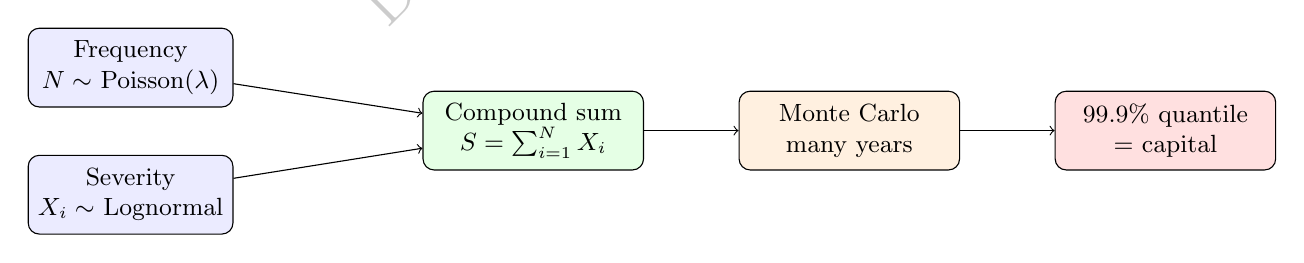
\begin{tikzpicture}[node distance=6mm and 12mm, every node/.style={font=\small}]
\node[draw, rounded corners, fill=blue!8, minimum width=2.6cm, minimum height=1cm, align=center] (freq) {Frequency\\ $N\sim$ Poisson$(\lambda)$};
\node[draw, rounded corners, fill=blue!8, minimum width=2.6cm, minimum height=1cm, align=center, below=of freq] (sev) {Severity\\ $X_i\sim$ Lognormal};
\node[draw, rounded corners, fill=green!10, minimum width=2.8cm, minimum height=1cm, align=center, right=2.4cm of freq, yshift=-8mm] (comp) {Compound sum\\ $S=\sum_{i=1}^N X_i$};
\node[draw, rounded corners, fill=orange!12, minimum width=2.8cm, minimum height=1cm, align=center, right=of comp] (mc) {Monte Carlo\\ many years};
\node[draw, rounded corners, fill=red!12, minimum width=2.8cm, minimum height=1cm, align=center, right=of mc] (cap) {99.9\% quantile\\ = capital};
\draw[->] (freq) -- (comp);
\draw[->] (sev) -- (comp);
\draw[->] (comp) -- (mc);
\draw[->] (mc) -- (cap);
\end{tikzpicture}
\end{lrbox}
\ifdim\wd\bookmeasuredbox<0.65\linewidth
\setlength{\bookcapwidth}{0.65\linewidth}
\else
\setlength{\bookcapwidth}{\wd\bookmeasuredbox}
\fi
\ffigbox[\bookcapwidth]{
\usebox{\bookmeasuredbox}
}{
\caption{The loss distribution approach: Monte Carlo convolves frequency and severity into an annual-loss distribution, and capital is read off its far tail}
\label{fig:oprisk-lda-pipeline}
}
\end{figure}

\section{Where Artificial Intelligence Enters}

Four distinct layers of machine learning sit on top of operational-risk data, each answering a different question.

\subsection{Where Artificial Intelligence Enters: Four Layers}
\label{sec:oprisk-ai-layers}

Nothing in the loss-distribution machinery above used machine learning, and that is deliberate: the frequency-severity core of operational-risk quantification is largely a small-data, distributional problem to which modern AI adds little. Artificial intelligence contributes elsewhere, in four layers that sit around the loss-modeling core rather than inside it, shown in Figure~\ref{fig:oprisk-ai-layers}. Each corresponds to a different point on the timeline of an operational-risk event, from the leading indicators that precede it, through the near-misses and anomalies that presage it, to the incident record it leaves behind, and each reuses a family of methods this book has already developed.

\begin{figure}[htbp]
\centering
\begin{lrbox}{\bookmeasuredbox}
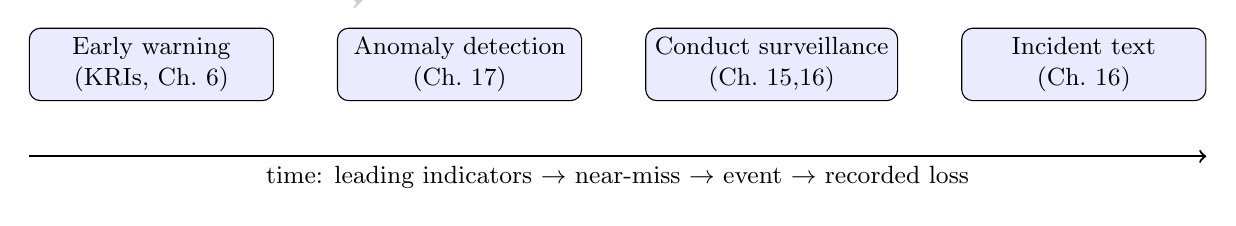
\begin{tikzpicture}[node distance=4mm, every node/.style={font=\small}]
\node[draw, rounded corners, fill=blue!8, minimum width=3.1cm, minimum height=0.9cm, align=center] (kri) {Early warning\\ (KRIs, Ch.~6)};
\node[draw, rounded corners, fill=blue!8, minimum width=3.1cm, minimum height=0.9cm, align=center, right=8mm of kri] (anom) {Anomaly detection\\ (Ch.~17)};
\node[draw, rounded corners, fill=blue!8, minimum width=3.1cm, minimum height=0.9cm, align=center, right=8mm of anom] (surv) {Conduct surveillance\\ (Ch.~15,16)};
\node[draw, rounded corners, fill=blue!8, minimum width=3.1cm, minimum height=0.9cm, align=center, right=8mm of surv] (text) {Incident text\\ (Ch.~16)};
\draw[->, thick] ([yshift=-7mm]kri.south west) -- ([yshift=-7mm]text.south east) node[midway, below] {time: leading indicators $\rightarrow$ near-miss $\rightarrow$ event $\rightarrow$ recorded loss};
\end{tikzpicture}
\end{lrbox}
\ifdim\wd\bookmeasuredbox<0.65\linewidth
\setlength{\bookcapwidth}{0.65\linewidth}
\else
\setlength{\bookcapwidth}{\wd\bookmeasuredbox}
\fi
\ffigbox[\bookcapwidth]{
\usebox{\bookmeasuredbox}
}{
\caption{Four layers where machine learning contributes, along the timeline of a loss event}
\label{fig:oprisk-ai-layers}
}
\end{figure}

\subsection{AI Layer 1: Text as the Primary Operational-Risk Data Source}
\label{sec:oprisk-text}

The single most abundant operational-risk data source inside a bank is not a table of losses; it is text. Incident reports, internal-audit findings, risk-and-control self-assessment narratives, customer complaints, and help-desk tickets accumulate continuously and describe operational events in far richer detail than any structured loss database captures. The problem is that this text is unstructured, and turning it into something a loss model can use, above all, sorting each incident into a Basel event type so that frequencies and severities can be estimated per category, is a text-classification task of the kind Chapter 16 developed.

Consider a minimal illustration in the spirit of Chapter 16's Naive Bayes classifier, distinguishing two event types from short incident descriptions: internal fraud (IF) and business disruption or system failure (SF). Table~\ref{tab:oprisk-nb} gives a tiny training set.

\begin{table}[htbp]
\centering
\begin{lrbox}{\bookmeasuredbox}
\begin{tabular}{p{3.0cm}p{9.5cm}}
\toprule
Event type & Incident descriptions (training) \\
\midrule
Internal fraud (IF) & ``trader hid unauthorized position''; ``employee falsified approval to hide loss''; ``unauthorized trade concealed by staff'' \\
System failure (SF) & ``batch system failed overnight settlement''; ``software deployment caused outage''; ``system outage delayed settlement'' \\
\bottomrule
\end{tabular}
\end{lrbox}
\ifdim\wd\bookmeasuredbox<0.65\linewidth
\setlength{\bookcapwidth}{0.65\linewidth}
\else
\setlength{\bookcapwidth}{\wd\bookmeasuredbox}
\fi
\floatbox[\capbot]{table}[\bookcapwidth]{
\usebox{\bookmeasuredbox}
}{
\caption{Training incidents for a two-class Naive Bayes event-type classifier}
\label{tab:oprisk-nb}
}
\end{table}

With equal class priors ($P(\text{IF}) = P(\text{SF}) = 0.5$), a vocabulary of $V = 24$ distinct words, and Laplace (add-one) smoothing, the classifier scores a new incident by summing log-probabilities word by word, just as in Chapter 16. For the smoothed likelihood of word $w$ in class $c$,
\begin{equation*}
P(w \mid c) = \frac{\text{count}(w, c) + 1}{\text{count}(c) + V},
\end{equation*}
where $\text{count}(c)$ is the total word count in class $c$. Classifying the new report ``unauthorized trade hidden by trader'' gives log-scores of about $-15.83$ for internal fraud and $-18.75$ for system failure; exponentiating and normalizing turns these into a posterior probability of \textbf{0.949} for internal fraud. The words \emph{unauthorized}, \emph{trade}, and \emph{trader} all appear in the fraud training incidents and none in the system-failure ones, so even though \emph{hidden} was never seen in training (and contributes only through smoothing), the classifier is decisive and correct.

At production scale the same idea, moved from a hand-checkable Naive Bayes to the TF-IDF representations and contextual embeddings of Chapter 16, does three jobs at once: it routes each incident to the right Basel category so the loss model of Section~\ref{sec:oprisk-lda} is fed clean per-category data; it clusters free-text root-cause narratives to surface recurring control weaknesses no single report would reveal; and it flags, from complaint text alone, the mis-selling and conduct issues that make up the ``clients, products and business practices'' event type, often the single largest source of operational losses at large banks.

The clustering job deserves emphasis, because it is where text analytics does something the structured loss database cannot. A bank's incidents are logged by whoever wrote them up, in inconsistent language, and the Basel category assigned at logging is often a coarse after-the-fact guess. Unsupervised topic modeling over the incident corpus, the same dimensionality-reduction impulse as Chapter 6's clustering, groups incidents by what actually happened rather than by how they were filed, and it routinely reveals that a scatter of separately logged ``minor'' incidents, a repeated reconciliation break, a recurring manual workaround, share a single underlying control failure that, uncorrected, is one bad day away from a large loss. Extracting a structured severity and root cause from each narrative, increasingly with the large language models of Chapter 16 rather than keyword rules, is what turns a pile of free text into the clean per-category frequency and severity data the loss model of Section~\ref{sec:oprisk-lda} silently assumes it was handed.

\subsection{AI Layer 2: Anomaly Detection for Near-Misses and Control Breaks}
\label{sec:oprisk-anomaly}

Waiting for a recorded loss is waiting too long. Many operational failures announce themselves first as \emph{anomalies}, a settlement process that suddenly takes an unusual path, a user account that touches systems it never normally touches, a trade booked outside its desk's usual pattern, well before they crystallize into a reportable loss. Because these near-misses are, by definition, deviations from normal behavior rather than examples of a labeled class, they are a natural fit for the unsupervised anomaly-detection methods of Chapter 17, above all the autoencoder\index{autoencoder}, which learns to reconstruct normal activity and flags whatever it reconstructs poorly.

The mechanism is the one Chapter 17 developed: train a model on a large sample of ordinary daily control-log feature vectors, then score each new vector by its reconstruction error, the squared distance between the vector and the model's attempt to reproduce it, and flag any observation whose error exceeds a high percentile of the normal distribution. In a stylized five-feature illustration where normal reconstruction errors follow the expected chi-square pattern, the 99th-percentile threshold sits at about $14.9$ (close to the theoretical chi-square value of $15.1$), and an injected anomalous vector representing a process break produces a reconstruction error of $35.5$, comfortably above the threshold and therefore flagged.

The single-vector result flatters the method, though, and a fuller test shows why. Applying the same 99th-percentile threshold (about $15.2$ in this run) to a test set of 500 normal observations and 50 genuinely anomalous ones, whose feature means are shifted only moderately rather than dramatically, gives the confusion matrix in Table~\ref{tab:oprisk-anomaly}: the detector catches 28 of the 50 anomalies (recall $0.56$) at a precision of $0.85$. The precision is respectable, but the recall is the sobering number: at a threshold strict enough to keep false alarms low, the detector misses nearly half of the moderate anomalies entirely. Loosening the threshold to catch more of them would flood the investigators with false positives, the same precision-recall trade-off Chapter 15 made central to fraud detection, and it is why anomaly detection is a triage tool that narrows where humans look rather than a complete substitute for their judgment.

\begin{table}[htbp]
\centering
\begin{lrbox}{\bookmeasuredbox}
\begin{tabular}{lcc}
\toprule
 & Flagged & Not flagged \\
\midrule
Truly anomalous (50) & 28 (true positive) & 22 (false negative) \\
Truly normal (500) & 5 (false positive) & 495 (true negative) \\
\bottomrule
\end{tabular}
\end{lrbox}
\ifdim\wd\bookmeasuredbox<0.65\linewidth
\setlength{\bookcapwidth}{0.65\linewidth}
\else
\setlength{\bookcapwidth}{\wd\bookmeasuredbox}
\fi
\floatbox[\capbot]{table}[\bookcapwidth]{
\usebox{\bookmeasuredbox}
}{
\caption{Anomaly detector at the 99th-percentile reconstruction-error threshold, on a test set of 500 normal and 50 anomalous observations}
\label{tab:oprisk-anomaly}
}
\end{table}

The same logic, at production scale and on real transaction, access, and trade logs, is what lets an operational-risk team catch a control failure while it is still a near-miss, the one point on the event timeline where intervention is cheapest, provided the team reads the recall number honestly and does not mistake a quiet alert queue for an absence of problems.

\subsection{AI Layer 3: Conduct and Rogue-Trading Surveillance}
\label{sec:oprisk-surveillance}

The Société Générale loss that opened this chapter belongs to a long line, Barings and Nick Leeson in 1995, Société Générale and Jérôme Kerviel in 2008, UBS and Kweku Adoboli in 2011, in which a single trader's concealed positions, undetected until far too late, produced a loss large enough to threaten the institution. Each is, in retrospect, a surveillance failure: the warning signs, unusual trade cancellations, positions inconsistent with stated limits, communications hinting at concealment, existed in the bank's own data and were simply not connected in time.

Conduct surveillance is where two of this book's threads converge on operational risk. The trade-pattern side is anomaly detection applied to a trader's own activity, the methods of Chapter 15's financial-crime models and Section~\ref{sec:oprisk-anomaly}'s reconstruction-error approach, now hunting for a book that no longer looks like its own history. The communications side is natural language processing applied to electronic communications, the e-comms surveillance systems that scan chat and email for the linguistic markers of collusion, concealment, or market manipulation, using the sentiment and classification machinery of Chapter 16. The 2012--2015 LIBOR and foreign-exchange manipulation cases, in which the incriminating evidence was largely trader chat, are the reason every major bank now runs NLP-based communications surveillance as a first-class operational-risk control rather than an afterthought.

A minimal illustration shows how the communications side works, using the same Naive Bayes machinery as Section~\ref{sec:oprisk-text}. Suppose a surveillance model is trained on two classes of short chat messages: ordinary business talk (``please confirm the trade details,'' ``the settlement date is tomorrow'') and messages exhibiting concealment markers (``keep this off the record,'' ``do not put this in writing,'' ``delete this message after reading''). Scoring the new message ``do not leave a trail on this,'' with a vocabulary of 36 words and equal priors, gives log-scores of about $-23.86$ for the suspicious class and $-28.99$ for the clean class, a posterior probability of \textbf{0.994} that the message warrants review. The words \emph{do}, \emph{not}, \emph{leave}, and \emph{trail} echo the concealment training examples closely enough that the classifier is nearly certain, the kind of first-pass triage that lets a human surveillance analyst focus on the small fraction of communications most likely to matter, from a daily volume no team could read in full.

The caveat parallels the fraud-detection lesson of Chapter 15: the base rate of genuine misconduct in trader communications is extremely low, so even a highly accurate classifier flags far more innocent messages than guilty ones, and a surveillance program's usefulness depends as much on ranking and prioritizing its alerts, and on the human review that follows them, as on the raw accuracy of the classifier itself.

The trade-pattern side of surveillance is where operational risk connects most directly to the market-microstructure material of Chapters 13 and 14. A rogue trader's book, by construction, stops looking like its own history: positions grow beyond stated limits, hedges that should offset a position are fictitious or absent, and the pattern of trade cancellations and amendments used to conceal the position departs from the desk's normal behavior. Each of these is detectable as an anomaly against the trader's own historical baseline, and the most effective surveillance systems fuse the two channels, a communications flag and a trading-pattern flag arriving together is far more informative than either alone, an application of the Bayesian-updating logic Chapter 1 introduced, in which two independent weak signals combine into one strong one. The persistent difficulty, common to every rogue-trading case in the historical record, is that the concealment is deliberate and adaptive: the trader knows the controls and works around them, which is why surveillance is an adversarial problem in which yesterday's detection rule is precisely what tomorrow's evasion is designed to defeat.

\subsection{AI Layer 4: Predictive Early Warning from Key Risk Indicators}
\label{sec:oprisk-kri}

The earliest point on the event timeline is before any anomaly at all, when only the \emph{conditions} that make a loss more likely are present. Operational-risk teams track these conditions as key risk indicators\index{key risk indicators}: measurable quantities such as staff overtime hours, system downtime, transaction volume spikes, and employee turnover that plausibly precede loss events. The predictive question, does this business unit's current indicator profile signal elevated loss risk next quarter, is a supervised classification problem of the kind Chapter 6 developed, and a logistic regression is the natural first model.

Consider the eight business units in Table~\ref{tab:oprisk-kri}, each described by three indicators, overtime hours (in hundreds), system downtime hours, and staff turnover percentage, and labeled by whether a major loss event followed in the next quarter. A logistic regression fit to this data (after standardizing the indicators so their coefficients are comparable) gives positive standardized coefficients on all three (about $0.82$ on overtime, $0.69$ on downtime, and $0.77$ on turnover), confirming that each is associated with higher loss probability, with overtime the strongest single signal.

\begin{table}[htbp]
\centering
\begin{lrbox}{\bookmeasuredbox}
\begin{tabular}{lcccc}
\toprule
Unit & Overtime (00s hrs) & Downtime (hrs) & Turnover (\%) & Loss event? \\
\midrule
1 & 12 & 2  & 8  & No \\
2 & 45 & 9  & 22 & Yes \\
3 & 18 & 3  & 10 & No \\
4 & 50 & 12 & 30 & Yes \\
5 & 8  & 1  & 5  & No \\
6 & 40 & 8  & 25 & Yes \\
7 & 22 & 4  & 12 & No \\
8 & 55 & 15 & 35 & Yes \\
\bottomrule
\end{tabular}
\end{lrbox}
\ifdim\wd\bookmeasuredbox<0.65\linewidth
\setlength{\bookcapwidth}{0.65\linewidth}
\else
\setlength{\bookcapwidth}{\wd\bookmeasuredbox}
\fi
\floatbox[\capbot]{table}[\bookcapwidth]{
\usebox{\bookmeasuredbox}
}{
\caption{Eight business units: key risk indicators and subsequent major-loss outcome}
\label{tab:oprisk-kri}
}
\end{table}

The fitted model then scores new units: a stressed unit running high on all three indicators receives a predicted loss probability of about \textbf{0.90}, while a calm unit low on all three receives about \textbf{0.07}, a spread wide enough to be genuinely useful for prioritizing where limited control-testing attention should go.

The caveat is one this book has raised before and that applies with particular force here. The moment a key risk indicator becomes a management target, staff have an incentive to manage the indicator rather than the underlying risk, and it ceases to measure what it once did, the Goodhart's Law\index{Goodhart's law} dynamic introduced in Chapter 1. A unit told that high overtime flags it for scrutiny can simply stop recording overtime. Predictive early-warning models are therefore best treated as one input to human judgment, monitored for the kind of gaming that would quietly hollow out their signal, rather than as automated verdicts.

\section{From Detection to Governance}

Detecting a control breach is only useful if something changes; this part covers prevention, the risks AI itself introduces, and validation.

\subsection{From Detection to Prevention: Process Mining}
\label{sec:oprisk-process-mining}

The four detection layers above catch operational failures as or after they happen; a fifth, more preventive use of data aims to remove the conditions that let them happen at all. Process mining\index{process mining} reconstructs how a business process actually ran, step by step, from the timestamped event logs that back-office systems generate automatically, and compares that reconstructed reality against how the process was designed to run. The operational-risk value is that the gaps between the two, a control step routinely skipped, an approval granted before its prerequisite, a transaction path that bypasses a four-eyes check, are the latent control weaknesses that eventually produce a loss, and they are visible in the logs long before any loss occurs.

Process mining is less glamorous than the machine-learning layers and uses simpler techniques, graph reconstruction and conformance checking rather than deep networks, but it targets the cheapest possible point of intervention: fixing a broken control before it is ever exploited. It pairs naturally with the anomaly detection of Section~\ref{sec:oprisk-anomaly}, which flags individual unusual events, by instead flagging systematic deviations in the process itself, and with robotic process automation, which, by executing routine steps deterministically, removes the human error that the ``execution, delivery and process management'' event type of Table~\ref{tab:oprisk-event-types} is built around, while introducing its own new automation-failure risk in exchange.

This preventive posture also reframes where the four AI layers deliver their value. Detection reduces the \emph{severity} of a loss by shortening the time between a failure and its discovery; prevention reduces the \emph{frequency} of loss events outright by removing the conditions that cause them. In the frequency-severity language of Section~\ref{sec:oprisk-lda}, the surveillance and anomaly layers act mostly on severity, catching an unfolding event sooner, while process mining, robotic automation, and the leading-indicator layer act on frequency, and a mature operational-risk program deliberately invests across both so that the loss distribution is pulled inward from both ends rather than only truncated at the tail.

\subsection{Entitlement Graphs and Segregation of Duties}\index{segregation of duties}\index{entitlement graph}
\label{sec:oprisk-entitlements}

The oldest operational-risk control of all is \emph{segregation of duties}: no one person should be able to both create a payee and pay it, or both enter a trade and confirm it, because a single individual holding both halves can complete a fraud without needing anyone's cooperation. Every rogue-trading case in Section~\ref{sec:oprisk-surveillance}'s list involved this control failing. Testing it sounds trivial, a matter of checking whether any user holds two conflicting permissions, and in a small system it is. What makes it hard at scale is that permissions are rarely granted to people directly. They are granted to roles, roles are nested inside other roles for administrative convenience, and a user inherits the transitive closure. The conflict is then a \emph{path} through the access graph, not an edge, and a check written over directly-granted permissions cannot see it.

Table~\ref{tab:oprisk-sod} makes the gap concrete on a deliberately small system: eight users, six granting roles, two composite roles that merely nest others (\texttt{AP\_MANAGER} contains the accounts-payable clerk and supervisor roles; \texttt{OPS\_ONCALL} contains treasury operations and static data), and four declared toxic permission pairs. Checking each user's directly-granted permissions flags exactly one user, \texttt{u3}, who visibly holds both halves of a conflict. Resolving the nested roles first and then applying the identical four-pair test flags four users. The three additional violations, \texttt{u4}, \texttt{u6}, and \texttt{u8}, are invisible to the direct check not because the test is wrong but because each user's conflicting permission arrives one hop away, through a composite role granted for an unrelated reason.

\begin{table}[htbp]
\centering
\begin{lrbox}{\bookmeasuredbox}
\begin{tabular}{llc}
\toprule
User & Conflicting pair held & Visible to a direct check? \\
\midrule
\texttt{u3} & create vendor $+$ approve payment & Yes \\
\texttt{u4} & create vendor $+$ approve payment & No, via \texttt{AP\_MANAGER} \\
\texttt{u6} & modify static data $+$ release payment & No, via \texttt{OPS\_ONCALL} \\
\texttt{u8} & create vendor $+$ release payment & No, via \texttt{OPS\_ONCALL} \\
\bottomrule
\end{tabular}
\end{lrbox}
\ifdim\wd\bookmeasuredbox<0.65\linewidth
\setlength{\bookcapwidth}{0.65\linewidth}
\else
\setlength{\bookcapwidth}{\wd\bookmeasuredbox}
\fi
\floatbox[\capbot]{table}[\bookcapwidth]{
\usebox{\bookmeasuredbox}
}{
\caption{Segregation-of-duties conflicts in an eight-user system. A pairwise check on directly-granted permissions finds one; following paths through nested roles finds four.}
\label{tab:oprisk-sod}
}
\end{table}

A ratio of four to one on eight users is not itself the finding; the point is that the missed fraction grows with the depth of role nesting, and real entitlement systems at large banks carry tens of thousands of users, thousands of roles, and nesting several levels deep, accumulated over decades of joiners, movers, and leavers whose permissions were added on each move and rarely removed. At that scale the same question becomes a genuine graph problem, and the network methods this book develops elsewhere apply directly: reachability queries of the kind Chapter 15's layering-network analysis uses to trace funds through intermediaries, now tracing authority through roles, and, where the toxic combinations are not all known in advance, the graph neural networks of Chapter 17 learning which access patterns resemble those that preceded past incidents. This is the cheapest intervention point in the entire chapter, since a conflict removed from the entitlement graph is a loss event that cannot occur through that route at all, as against the detection layers, which at best notice it sooner.

\subsection{Predictive Process Monitoring}\index{predictive process monitoring}
\label{sec:oprisk-predictive-process}

Conformance checking compares a process against its design after the fact. The natural extension is to ask, of a case still running, what is likely to happen to it next, which turns the event log into a sequence-prediction problem of the kind Chapters 7 and 16 develop. Given the prefix of activities a payment or a trade settlement has completed so far, together with their timestamps and attributes, a model predicts the next activity, the remaining time to completion, or the probability that the case ends in a breach, an exception, or a manual write-off. Recurrent and attention-based architectures are the standard tools, since the informative signal is usually the \emph{order} of steps and the gaps between them rather than any single step in isolation, which is precisely the structure Chapter 16's self-attention mechanism was built to exploit.

The operational-risk value is that it converts process data from a diagnostic record into a leading indicator at the level of the individual case, complementing the business-unit-level indicators of Section~\ref{sec:oprisk-kri}: a settlement predicted to breach its deadline can be escalated while there is still time to act on it. The caveats are the familiar ones and apply with full force. The training labels come from historical cases whose outcomes were themselves shaped by whatever interventions the firm was already making, so a model that learns from them is learning the process as operated rather than the process as designed; and a prediction that triggers an intervention destroys the very outcome it predicted, making honest evaluation harder than a backtest suggests, which is the same reflexivity Section~\ref{sec:oprisk-kri} raised about key risk indicators and which the next section takes up as a general problem.

\subsubsection*{The Reflexive Turn: Artificial Intelligence as a Source of Operational Risk}
\label{sec:oprisk-reflexive}

Every method in the four layers above uses AI to \emph{manage} operational risk. But deploying those same models is itself an operational activity, with its own failure modes, and so artificial intelligence is not only a tool against operational risk but increasingly a source of it. This reflexive point is not a rhetorical flourish; it is now an explicit category in most banks' operational-risk taxonomies.

The oldest form is model risk\index{model risk}, the risk that a model is simply wrong, or is used outside the conditions it was built for, which this book has flagged from Chapter 6 onward and which regulators treat as an operational-risk discipline in its own right. A credit or trading model whose assumptions are quietly violated by a changing environment produces losses that are, in the end, operational: a failure of an internal system. The monitoring apparatus of Chapter 18, population-stability indices, drift detection, and the explainability tools that let a human challenge a model's outputs, is best understood as an operational-risk control for models, the mechanism by which model risk is detected before it becomes a loss.

Generative AI adds newer failure modes that did not exist when the Basel event types were written. A large language model that fabricates a plausible but false answer (hallucination), a system manipulated into ignoring its instructions through adversarial input (prompt injection), and a critical dependence on a single external model vendor whose service can change or fail (third-party and concentration risk) are all operational risks in the strict Basel sense, failures of systems, processes, or external parties, even though no traditional operational-risk framework anticipated them.

A sharper version of the same concern arrives once the model stops merely producing text and starts \emph{taking actions}. The LLM agents with tool use that Chapter 16 describes do not draft an answer for a person to read and check; they call functions, and those functions can submit an order, release a payment, open a ticket, or change a configuration. That difference is not one of degree. Every control in the four detection layers above assumes a window between a failure and its consequences, the window in which an anomaly is a near-miss rather than a loss, and an agent that acts closes that window by construction: the first observable evidence is an executed transaction, not a proposal anyone declined. Two further properties compound it. An agent granted the entitlements it needs to be useful across several systems is a segregation-of-duties breach of the kind Section~\ref{sec:oprisk-entitlements} exists to prevent, since it holds both halves of a conflicting pair and, unlike a human, will never hesitate at the second half; and because it acts at machine speed and without fatigue, a single flawed instruction propagates across thousands of cases before the daily control report that would have caught it is even generated. The controls that follow are correspondingly conventional and worth stating plainly, because they are the ones the operational-risk framework already knows how to write: scope each agent's permissions to the minimum its task requires rather than to the maximum its convenience suggests, keep a human approval step on any action that moves money or commits the firm, log every tool call as a first-class auditable event, and impose hard rate and value limits so that a failure is bounded before anyone notices it. None of this is novel risk management. It is the same segregation, authorization, and limit discipline banks have applied to human traders since Barings, applied to a non-human actor that the existing control framework does not yet recognize as one.

A concrete example makes the mapping vivid. Suppose a bank deploys a retrieval-augmented assistant, of the kind Chapter 16 described, to draft responses to client queries about their products. If the model confidently states an incorrect fee or an inaccurate contractual term, and a client acts on it, the resulting loss is not a market or credit loss; it is a ``clients, products and business practices'' operational loss, indistinguishable in its consequences from a human adviser's mis-statement, but arriving at a scale and speed no human adviser could match, since the same flawed model answers thousands of queries before anyone notices. The controls are correspondingly operational: retrieval grounding to reduce fabrication, human review of high-stakes outputs, logging for after-the-fact audit, and the drift monitoring of Chapter 18 to catch a model whose behavior degrades after a vendor update. The lesson is that embedding AI does not create a new \emph{kind} of risk so much as a new, faster \emph{channel} for the operational risks the framework already names. As institutions embed the generative methods of Chapter 16 into research, client service, and compliance workflows, mapping these new failure modes onto the operational-risk framework, and building controls for them, becomes part of the operational-risk function's job.

\subsubsection*{Regulation: Why Artificial Intelligence Lives in Management, Not Capital}
\label{sec:oprisk-regulation}

There is a striking regulatory irony at the center of this chapter. Just as machine learning was maturing into a serious tool for operational risk, the Basel Committee moved decisively \emph{away} from letting banks use their own internal models to set operational-risk \emph{capital}. The Advanced Measurement Approach, which had permitted sophisticated internal loss-distribution models of the kind Section~\ref{sec:oprisk-lda} describes, was retired in the Basel III finalization in favor of the Standardized Measurement Approach, which ties capital mechanically to a size-based ``business indicator'' adjusted by the bank's own historical loss experience, the same philosophy as the Basic Indicator Approach Chapter 9 described, chosen for the same reason: the events are too heterogeneous and too sparse for regulators to trust any single institution's internal model of the tail.

The consequence is clarifying rather than discouraging. Because regulatory operational-risk capital is now formulaic, the value of the machinery in this chapter, the loss-distribution model and, above all, the four AI layers, lies in \emph{managing} operational risk rather than in setting the regulatory number: in reducing the frequency and severity of loss events through earlier detection, better surveillance, and sharper prioritization, and in informing a bank's own internal economic-capital view even where it no longer drives the regulatory one. Artificial intelligence's home in operational risk is the risk-management function, not the capital calculation, and that is exactly where its comparative advantage, unstructured data and rare-pattern detection, actually lies. Model risk itself remains squarely within supervisory scope through model-governance expectations such as the U.S. Federal Reserve's SR 11-7 guidance, which is why the reflexive controls of Section~\ref{sec:oprisk-reflexive} are not optional.

\subsubsection*{Validating and Backtesting Operational-Risk Models}
\label{sec:oprisk-validation}

Every model in this chapter must itself be validated, and operational risk makes validation unusually hard for the same reason it makes modeling hard: the events are too rare to backtest in the ordinary sense. A market-risk Value at Risk model can be backtested against roughly 250 daily outcomes a year, as Chapter 8 described, so a 99\% model should be breached about two or three times annually and a wildly miscalibrated one is caught quickly. A 99.9\% operational-risk capital model, by contrast, makes a prediction about a once-in-a-thousand-year loss that no institution will ever observe often enough to test directly. Validation therefore leans on indirect checks: goodness-of-fit tests on the severity distribution, sensitivity analysis to the assumed severity and frequency distributions, benchmarking against external loss data, and structured challenge of the scenario-analysis judgments that drive the tail.

The AI layers, by contrast, are far more testable, and should be held to the same standards as any other model in this book. An incident classifier has a confusion matrix (Chapter 6); an anomaly detector has a precision-recall trade-off measured against injected or historical anomalies (Chapter 15); an early-warning model has an out-of-sample discriminatory-power measure such as the AUC of Chapter 9. Holding these models to that standard, rather than trusting them because they happen to address an important problem, is itself part of the model-risk discipline of Section~\ref{sec:oprisk-reflexive}: an unvalidated surveillance model that quietly stops working is not a safeguard against operational risk but a new instance of it.

That said, ``more testable'' should not be read as ``straightforwardly testable,'' because for the surveillance layer in particular the labels needed to compute any of those metrics barely exist, and the ones that do exist are selected in a way that flatters the model. Confirmed misconduct is not merely rare; it is rare \emph{and} observed only where some control already caught it. A recall figure computed against a bank's history of confirmed rogue-trading cases is therefore recall against the events the current surveillance system, or an auditor, or a market move, happened to expose, and it is silent about the ones that were concealed successfully, which are precisely the population the model exists to find. A model can post an excellent recall on that sample while being systematically blind to the concealment techniques that work. Chapter 9 meets the identical structure in credit under the name reject inference, where a scorecard can only be validated on applicants it approved and never on the ones it turned away, and the response here borrows the same instincts: evaluate against deliberately injected synthetic scenarios that encode known evasion patterns as well as against historical cases, treat the alert queue's precision, which \emph{is} cleanly measurable from investigator dispositions, as the more trustworthy of the two numbers, and read any reported recall as an upper bound rather than an estimate. The honest summary is that the detection layers can be validated well against false positives and only weakly against false negatives, which is a further reason, alongside the base-rate problem of Section~\ref{sec:oprisk-surveillance}, to treat a quiet alert queue as an ambiguous signal rather than a reassuring one.

\section{Case Vignette: The 2012 JPMorgan ``London Whale''}
\label{sec:oprisk-vignette}

In 2012 JPMorgan Chase lost more than \$6 billion in its Chief Investment Office through a portfolio of credit derivatives that grew so large a single trader earned the nickname ``the London Whale.''\index{London Whale (JPMorgan)} The loss is usually told as a risk-management story, and it was, but at its core it was operational. A spreadsheet-based Value at Risk model used to monitor the position contained a formula error that understated its risk; the position had grown beyond what its stated strategy could justify; and internal warnings were not escalated in time. Every element, a flawed model, a control that failed to bind, an escalation process that did not function, is an operational-risk failure in the Basel sense, not a market-risk one, even though the loss ultimately materialized through market prices.

The episode is a compact illustration of this chapter's whole argument. The model error is model risk (Section~\ref{sec:oprisk-reflexive}), of the kind Chapter 18's validation and monitoring tools exist to catch. The unnoticed drift of the position away from its mandate is a near-miss anomaly (Section~\ref{sec:oprisk-anomaly}) that trade-pattern surveillance is designed to surface. The failure to escalate is the kind of process breakdown that leading indicators (Section~\ref{sec:oprisk-kri}) and incident analysis (Section~\ref{sec:oprisk-text}) are meant to make visible. No single AI system would have prevented the London Whale, but each layer of this chapter maps directly onto a point at which the failure could have been caught earlier, which is precisely why operational-risk management is best understood as a portfolio of overlapping detection layers rather than a single model.

The aftermath reinforces the chapter's regulatory theme. JPMorgan ultimately paid roughly \$920 million in coordinated regulatory settlements over the episode, an amount that dwarfs the capital any internal model would plausibly have held against this specific risk, and the enforcement findings centered not on the size of the market bet but on the control and governance failures around it: risk limits that were breached and then re-calibrated rather than enforced, a valuation process that masked losses, and a model change that was implemented without adequate validation. That emphasis is why, as Section~\ref{sec:oprisk-regulation} argued, the supervisory response to operational risk runs through governance expectations and model-risk discipline rather than through a capital formula, and why the value of this chapter's tools lies in strengthening the controls whose failure, not the trade itself, turned a large loss into a far larger one.

\section{Challenges in Operational Risk Modeling}
\label{sec:oprisk-challenges}

The difficulties that make operational risk awkward are not incidental; they are structural, and honest practice acknowledges them rather than modeling past them.

\textbf{Data scarcity and the unquantifiable tail.} The largest operational losses are, by definition, the rarest, so the very events that dominate the capital number are the ones about which there is least data. No amount of machine learning manufactures tail observations that do not exist, and a genuinely unprecedented event, a first-of-its-kind cyberattack, a novel misconduct scheme, is closer to the Knightian uncertainty of Chapter 1 than to the estimable risk any model assumes.

\textbf{Reporting and survivorship bias.} Loss databases record what was noticed and reported; near-misses, silently absorbed small losses, and the losses of firms that did not survive are all systematically missing, biasing any fitted frequency and severity downward in ways no purely statistical correction can fully repair.

\textbf{Alert fatigue.} Every detection layer in this chapter produces false positives, and the base-rate reasoning of Chapter 15 applies in full: when true events are rare, even an accurate detector generates far more false alarms than genuine catches, and a surveillance system that overwhelms its investigators is, in practice, no surveillance at all.

\textbf{Model-on-model risk.} Using AI to manage operational risk adds models whose own failures are operational risks, so the controls of Section~\ref{sec:oprisk-reflexive} must extend to the very models built to detect operational failures, a regress that is manageable but never fully closed.

\textbf{Gaming and reflexivity.} As the Goodhart dynamic of Section~\ref{sec:oprisk-kri} shows, indicators and controls that become targets can lose their meaning, so operational-risk models require ongoing revalidation against the possibility that the behavior they measure has adapted to their existence.

\textbf{The pace of new failure modes.} The event types in Table~\ref{tab:oprisk-event-types} were fixed years before generative AI, cloud concentration, or large-scale ransomware became material, and the pace at which technology creates genuinely new operational-risk channels now outruns the frameworks meant to catalog them. A framework that can only manage the risks it has already named is structurally behind, which is why the reflexive, continuously-monitored posture of Section~\ref{sec:oprisk-reflexive} matters more in operational risk than the one-time model sign-off that suffices elsewhere.

\section{Key Takeaways}

\begin{itemize}
\item Operational risk is the risk of loss from failed internal processes, people, systems, or external events, distinct from the market risk of Chapter 8 and the credit risk of Chapter 9, and structurally harder to model because its events are rare, heavy-tailed, heterogeneous, and under-reported.
\item The four data elements are combined, not pooled: a Gamma-Poisson credibility blend weights internal history against external and scenario data through a single factor $Z=n/(n+\beta)$, and in the worked example it turned a thin internal estimate of $8.4$ events a year into the $\lambda=12$ the loss model uses, a bank relying on internal data alone understating its capital by about $15\%$.
\item The classical loss distribution approach builds annual loss from a Poisson frequency and a lognormal severity by Monte Carlo; in the worked example, the 99.9\% capital quantile was about seven times the expected loss, so operational-risk capital is overwhelmingly a tail problem.
\item Operational-risk capital is dominated by the severity tail rather than the event frequency or the average loss, so modeling that tail well, with heavy-tailed and extreme-value methods, is the central actuarial difficulty and the place sparse data hurts most.
\item Artificial intelligence contributes in four layers around the loss-modeling core, incident-text classification (Chapter 16), anomaly detection for near-misses (Chapter 17), conduct and rogue-trading surveillance (Chapters 15--16), and predictive early warning from key risk indicators (Chapter 6), not by replacing the actuarial loss model.
\item Deploying AI is itself an operational activity: model risk, drift, and generative-AI failure modes such as hallucination and prompt injection are operational risks in their own right, and the monitoring tools of Chapter 18 are their controls.
\item Because Basel retired internal-model operational-risk capital in favor of a size-based formula, AI's home in operational risk is management and detection, exactly where its strengths lie, rather than the regulatory capital calculation.
\item Prevention beats detection: process mining, entitlement-graph analysis, and predictive process monitoring remove the conditions for a loss rather than shortening the time to notice one, and because permissions are inherited through nested roles, a segregation-of-duties conflict is a path through the access graph rather than an edge, invisible to a pairwise check.
\item An AI system that \emph{acts} rather than merely drafts is a different operational risk from one that generates text: it closes the detection window the four layers depend on, and holds conflicting entitlements by construction, so it needs the scoping, authorization, logging, and limit controls banks have applied to human traders since Barings.
\item The AI layers must themselves be validated with the same tools as any other model, confusion matrices, precision-recall curves, and out-of-sample discrimination, because an unmonitored surveillance or early-warning model that silently stops working is not a control against operational risk but a fresh source of it.
\item Those validations are far stronger against false positives than false negatives: confirmed-misconduct labels exist only where a control already caught something, the same reject-inference structure Chapter 9 meets in credit, so a reported surveillance recall is an upper bound and a quiet alert queue is ambiguous rather than reassuring.
\end{itemize}

\section{Suggested Exercises}

\begin{enumerate}
\item Using the loss distribution approach with $\lambda = 8$ events per year and Lognormal$(\mu=11, \sigma=1.2)$ severities, simulate the annual loss distribution and estimate the expected loss and the 99.9\% capital quantile. By what multiple does the capital exceed the expected loss, and how does that multiple change if you raise $\sigma$ to $1.6$?
\item Explain, in terms of the frequency and severity components, why two business lines with the same expected annual operational loss can require very different amounts of capital. Which component does raising the severity $\sigma$ affect, and why does it move the 99.9\% quantile more than the mean?
\item Extend the two-class Naive Bayes classifier of Section~\ref{sec:oprisk-text} to a third event type (for example, external fraud) with three new training incidents, and classify a new report of your choosing. Show the effect of Laplace smoothing on a word that appears in only one class.
\item Using the key-risk-indicator logistic regression of Section~\ref{sec:oprisk-kri}, explain why standardizing the indicators before fitting makes the coefficients comparable across indicators, and describe one way a business unit could game each of the three indicators without reducing its actual operational risk.
\item Explain why an anomaly detector with a precision of 0.85 but a recall of only 0.56, as in Table~\ref{tab:oprisk-anomaly}, can still be operationally valuable, and describe the concrete consequence, in analyst workload and in missed events, of lowering its threshold to raise recall to 0.90.
\item Using Section~\ref{sec:oprisk-credibility}'s credibility blend, recompute $\hat\lambda$ when the scenario workshop's view is held with strength $\beta = 8$ years rather than $3$, holding the internal $42$ events over $5$ years and $\lambda_{\text{prior}}=18$ fixed. Report the new credibility factor $Z$ and blended frequency, re-run the loss simulation at that frequency, and explain why a supervisor might be uncomfortable letting a bank choose $\beta$ for itself.
\item Section~\ref{sec:oprisk-credibility} showed that using internal loss data alone understates the 99.9\% capital quantile by about $15\%$ for this business line. Explain why the understatement is smaller in percentage terms than the corresponding gap in \emph{expected} loss, referring to how frequency and severity each enter the compound sum, and say what this implies for a business line whose severity $\sigma$ is larger.
\item Add a ninth user to Table~\ref{tab:oprisk-sod}'s system who holds the \texttt{TRADE\_ENTRY} role plus a new composite role containing \texttt{TRADE\_CONFIRM}, and confirm that the direct check misses the resulting conflict while the path-based check finds it. Then describe one realistic way an entitlement graph accumulates such conflicts without anyone making an obviously wrong decision.
\item Section~\ref{sec:oprisk-validation} argues that a surveillance model's reported recall should be read as an upper bound. Construct a small numerical illustration: assume 10 genuine misconduct episodes occurred, the existing controls exposed 4 of them, and a new model flags 3 of those 4. State the recall the bank would report, the recall against all 10, and explain which of the two a model validator can actually observe.
\item \textbf{Challenge (real data).} Public enforcement actions are a rich, freely available source of operational-loss narratives. Download a sample of settlement or enforcement-action texts (for example, from the U.S. Securities and Exchange Commission's litigation releases or the Consumer Financial Protection Bureau's enforcement database), label each by Basel event type, and train a text classifier (TF-IDF plus logistic regression, or the embedding methods of Chapter 16) to predict the event type from the narrative. Report its confusion matrix, and discuss which event types are hardest to separate and why.
\end{enumerate}

\section{Further Reading}

\begin{itemize}
\item Hull, \emph{Risk Management and Financial Institutions}. Includes a clear introductory treatment of operational risk and its regulatory capital, complementing the market- and credit-risk chapters cited in Chapters 8 and 9.
\item Cruz, Peters, and Shevchenko, \emph{Fundamental Aspects of Operational Risk and Insurance Analytics}. A thorough treatment of the loss distribution approach, frequency-severity modeling, and the extreme-value methods for the severity tail.
\item McNeil, Frey, and Embrechts, \emph{Quantitative Risk Management: Concepts, Techniques and Tools}. A standard graduate reference spanning market, credit, and operational risk, and the extreme-value methods for heavy-tailed losses.
\item Board of Governors of the Federal Reserve System, \emph{Supervisory Guidance on Model Risk Management} (SR 11-7). The foundational supervisory statement treating model risk as an operational-risk discipline, underlying Sections~\ref{sec:oprisk-reflexive} and~\ref{sec:oprisk-regulation}.
\item Shevchenko, \emph{Modelling Operational Risk Using Bayesian Inference}. A book-length treatment of the problem Section~\ref{sec:oprisk-credibility} works in miniature, combining internal loss data, external data, and expert scenario judgment into a single frequency and severity estimate.
\item van der Aalst, \emph{Process Mining: Data Science in Action}. The standard reference for the event-log reconstruction and conformance checking of Section~\ref{sec:oprisk-process-mining}, and for the predictive extensions of Section~\ref{sec:oprisk-predictive-process}.
\end{itemize}

\end{document}

